\documentclass[10pt,fleqn]{article}
\newcommand{\name}[1]{\def\psettitlename{#1}}
\newcommand{\course}[1]{\def\psettitlecourse{#1}}
\newcommand{\rsection}[1]{\def\psettitlersection{#1}}
\newcommand{\psetnum}[1]{\def\psettitlepsetnum{#1}}
%\usepackage[journal=rsc]{chemstyle}
%\usepackage{mhchem}
\usepackage{amsmath}
\usepackage{amssymb}
\usepackage{amsfonts}
\usepackage{esint}
\usepackage{bbm}
\usepackage{amscd}
\usepackage{picinpar}
\usepackage[pdftex]{graphicx}
\usepackage{tikz}
\usepackage{indentfirst}
\usepackage{wrapfig}
\usepackage{units}
\usepackage{textcomp}
\usepackage[utf8x]{inputenc}
% \usepackage{feyn}
\usepackage{feynmp}
\usetikzlibrary{
  arrows,
  calc,
  decorations.pathmorphing,
  decorations.pathreplacing,
  decorations.markings,
  fadings,
  positioning,
  shapes
}

\DeclareGraphicsRule{*}{mps}{*}{}
\newcommand{\ud}{\mathrm{d}}
\newcommand{\ue}{\mathrm{e}}
\newcommand{\ui}{\mathrm{i}}
\newcommand{\res}{\mathrm{Res}}
\newcommand{\Tr}{\mathrm{Tr}}
\newcommand{\dsum}{\displaystyle\sum}
\newcommand{\dprod}{\displaystyle\prod}
\newcommand{\dlim}{\displaystyle\lim}
\newcommand{\dint}{\displaystyle\int}
\newcommand{\fsno}[1]{{\!\not\!{#1}}}
\newcommand{\eqar}[1]
{
  \begin{align*}
    #1
  \end{align*}
}
\newcommand{\texp}[2]{\ensuremath{{#1}\times10^{#2}}}
\newcommand{\dexp}[2]{\ensuremath{{#1}\cdot10^{#2}}}
\newcommand{\eval}[2]{{\left.{#1}\right|_{#2}}}
\newcommand{\paren}[1]{{\left({#1}\right)}}
\newcommand{\lparen}[1]{{\left({#1}\right.}}
\newcommand{\rparen}[1]{{\left.{#1}\right)}}
\newcommand{\abs}[1]{{\left|{#1}\right|}}
\newcommand{\sqr}[1]{{\left[{#1}\right]}}
\newcommand{\crly}[1]{{\left\{{#1}\right\}}}
\newcommand{\angl}[1]{{\left\langle{#1}\right\rangle}}
\newcommand{\tpdiff}[4][{}]{{\paren{\frac{\partial^{#1} {#2}}{\partial {#3}{}^{#1}}}_{#4}}}
\newcommand{\tpsdiff}[4][{}]{{\paren{\frac{\partial^{#1}}{\partial {#3}{}^{#1}}{#2}}_{#4}}}
\newcommand{\pdiff}[3][{}]{{\frac{\partial^{#1} {#2}}{\partial {#3}{}^{#1}}}}
\newcommand{\diff}[3][{}]{{\frac{\ud^{#1} {#2}}{\ud {#3}{}^{#1}}}}
\newcommand{\psdiff}[3][{}]{{\frac{\partial^{#1}}{\partial {#3}{}^{#1}} {#2}}}
\newcommand{\sdiff}[3][{}]{{\frac{\ud^{#1}}{\ud {#3}{}^{#1}} {#2}}}
\newcommand{\tpddiff}[4][{}]{{\left(\dfrac{\partial^{#1} {#2}}{\partial {#3}{}^{#1}}\right)_{#4}}}
\newcommand{\tpsddiff}[4][{}]{{\paren{\dfrac{\partial^{#1}}{\partial {#3}{}^{#1}}{#2}}_{#4}}}
\newcommand{\pddiff}[3][{}]{{\dfrac{\partial^{#1} {#2}}{\partial {#3}{}^{#1}}}}
\newcommand{\ddiff}[3][{}]{{\dfrac{\ud^{#1} {#2}}{\ud {#3}{}^{#1}}}}
\newcommand{\psddiff}[3][{}]{{\frac{\partial^{#1}}{\partial{}^{#1} {#3}} {#2}}}
\newcommand{\sddiff}[3][{}]{{\frac{\ud^{#1}}{\ud {#3}{}^{#1}} {#2}}}
\usepackage{fancyhdr}
\usepackage{multirow}
\usepackage{fontenc}
%\usepackage{tipa}
\usepackage{ulem}
\usepackage{color}
\usepackage{cancel}
\newcommand{\hcancel}[2][black]{\setbox0=\hbox{#2}%
\rlap{\raisebox{.45\ht0}{\textcolor{#1}{\rule{\wd0}{1pt}}}}#2}
\pagestyle{fancy}
\setlength{\headheight}{67pt}
\fancyhead{}
\fancyfoot{}
\fancyfoot[C]{\thepage}
\fancyhead[R]
{
\psettitlename \\
\psettitlecourse{} Problem Set \psettitlepsetnum \\
\ifx\psettitlersection\empty
\else
Recitation Section \psettitlersection
\fi
}
\renewcommand{\footruleskip}{0pt}
\renewcommand{\headrulewidth}{0.4pt}
\renewcommand{\footrulewidth}{0pt}
\addtolength{\hoffset}{-1.3cm}
\addtolength{\voffset}{-2cm}
\addtolength{\textwidth}{3cm}
\addtolength{\textheight}{2.5cm}
\renewcommand{\footskip}{10pt}
\setlength{\headwidth}{\textwidth}
\setlength{\headsep}{20pt}
\setlength{\marginparwidth}{0pt}
\parindent=0pt
\psetnum{3}
\course{8.422}
\rsection{1}
\name{Yichao Yu}
\renewcommand{\thesection}{\arabic{section}.}
\renewcommand{\thesubsection}{(\alph{subsection})}
\renewcommand{\thesubsubsection}{\roman{subsubsection}.}

\begin{document}
\section{}
\subsection{}
\eqar{
  H=&\hbar\omega b^\dagger b+\ui\hbar\Lambda\paren{{b^\dagger}^2+b^2}\\
  \diff{b}{t}=&\frac{\ui}{\hbar}\sqr{H, b}+\pdiff{b}{t}\\
  =&\sqr{\ui\omega b^\dagger b-\Lambda{b^\dagger}^2, b}+\ui\omega b\\
  =&2\Lambda b^\dagger\\
  \diff{b^\dagger}{t}=&2\Lambda b
}
\subsection{}
\eqar{
  \vec E=&\ui\mathcal{E}_\omega\vec\varepsilon\paren{b\ue^{\ui\paren{\vec k\cdot\vec r-\omega t}}-b^\dagger\ue^{-\ui\paren{\vec k\cdot\vec r-\omega t}}}\\
  =&\ui\mathcal{E}_\omega\vec\varepsilon\paren{b\cos\paren{\vec k\cdot\vec r-\omega t}+\ui b\sin\paren{\vec k\cdot\vec r-\omega t}-b^\dagger\cos\paren{\vec k\cdot\vec r-\omega t}+\ui b^\dagger\sin\paren{\vec k\cdot\vec r-\omega t}}\\
  =&-2\mathcal{E}_\omega\vec\varepsilon\paren{\frac{b-b^\dagger}{2\ui}\cos\paren{\vec k\cdot\vec r-\omega t}+\frac{b+b^\dagger}{2}\sin\paren{\vec k\cdot\vec r-\omega t}}\\
  =&-2\mathcal{E}_\omega\vec\varepsilon\paren{b_Q\cos\paren{\vec k\cdot\vec r-\omega t}+b_P\sin\paren{\vec k\cdot\vec r-\omega t}}\\
  \diff{b_{\pm}}{t}\equiv&\diff{b\pm b^\dagger}{t}\\
  =&2\Lambda b^\dagger\pm2\Lambda b\\
  =&\pm2\Lambda b_\pm\\
  \diff{b_P}{t}=&2\Lambda b_P\\
  \diff{b_Q}{t}=&-2\Lambda b_Q\\
  \intertext{Therefore}
  b_P=&\ue^{2\Lambda t}b_{P0}\\
  b_Q=&\ue^{-2\Lambda t}b_{Q0}\\
  b=&b_P+\ui b_Q\\
  =&\ue^{2\Lambda t}b_{P0}+\ui\ue^{-2\Lambda t}b_{Q0}\\
  =&b_0\cosh2\Lambda t+b_0^\dagger\sinh2\Lambda t\\
  b^\dagger=&b_0^\dagger\cosh2\Lambda t+b_0\sinh2\Lambda t
}
\subsection{}
\eqar{
  \angl{N}=&\langle0|b^\dagger b|0\rangle\\
  =&\langle0|\paren{b_0^\dagger\cosh2\Lambda t+b_0\sinh2\Lambda t}\paren{b_0\cosh2\Lambda t+b_0^\dagger\sinh2\Lambda t}|0\rangle\\
  =&\sinh^22\Lambda t\\
  \Delta b_P=&\ue^{2\Lambda t}\Delta b_{P0}\\
  =&\frac12\ue^{2\Lambda t}\\
  \Delta b_Q=&\ue^{-2\Lambda t}\Delta b_{Q0}\\
  =&\frac12\ue^{-2\Lambda t}
}
The state is squeezed in $Q$ direction while the product of the uncertainty in $P$ and $Q$ remains the same.
\subsection{}
Under the transformation $U=\ue^{\ui\omega t a^\dagger a}$
\eqar{
  UaU^\dagger=&\ue^{\ui\omega t a^\dagger a}a\ue^{-\ui\omega t a^\dagger a}\\
  =&\sum_N\frac{\paren{\ui\omega t}^N}{N!}\sqr{a^\dagger a, a}_N\\
  =&\ue^{-\ui\omega t}a\\
  Ua^\dagger U^\dagger=&\ue^{\ui\omega t}a^\dagger\\
  \diff{}{t}|\psi'\rangle=&\diff{}{t}U|\psi\rangle\\
  =&\diff{U}{t}|\psi\rangle+U\diff{}{t}|\psi\rangle\\
  =&\diff{\ue^{\ui\omega t a^\dagger a}}{t}|\psi\rangle+\frac{U}{\ui\hbar}H|\psi\rangle\\
  =&\ui\omega a^\dagger a|\psi'\rangle+\frac{1}{\ui\hbar}UHU^\dagger |\psi'\rangle\\
  =&\Lambda U\paren{{a^\dagger}^2\ue^{-2\ui\omega t}-a^2\ue^{2\ui\omega t}}U^\dagger |\psi'\rangle\\
  =&\Lambda\paren{{a^\dagger}^2-a^2}|\psi'\rangle\\
  \intertext{Therefore, the state $|\psi'\rangle$ is transforming as}
  &\ue^{\Lambda t\paren{{a^\dagger}^2-a^2}}
  \intertext{where}
  \varepsilon=&-2\Lambda t
}

\subsection{}
\subsubsection{}
\includegraphics[width=10cm]{{1e1_0.2}.png}\\
\includegraphics[width=10cm]{{1e1_1.2}.png}\\
\includegraphics[width=10cm]{{1e1_4}.png}
\subsubsection{}
$\beta=\ui$\\
\includegraphics[width=10cm]{{1e2_0.2}.png}\\
\includegraphics[width=10cm]{{1e2_1.2}.png}\\
\includegraphics[width=10cm]{{1e2_4}.png}
\subsubsection{}
$\beta=\ui$\\
\includegraphics[width=10cm]{{1e3_0.2}.png}\\
\includegraphics[width=10cm]{{1e3_1.2}.png}\\
\includegraphics[width=10cm]{{1e3_4}.png}

Weither a phase or number squeezed state is created depends on the initial state.

\section{}
\subsection{}
\eqar{
  \angl{N^2}=&\langle0|b^\dagger bb^\dagger b|0\rangle\\
  =&\langle0|\paren{b_0^\dagger\cosh\varepsilon+b_0\sinh\varepsilon}\paren{b_0\cosh\varepsilon+b_0^\dagger\sinh\varepsilon}\\
  &\paren{b_0^\dagger\cosh\varepsilon+b_0\sinh\varepsilon}\paren{b_0\cosh\varepsilon+b_0^\dagger\sinh\varepsilon}|0\rangle\\
  =&\sinh^2\varepsilon\langle0|\paren{b_0^2\cosh\varepsilon+b_0b_0^\dagger\sinh\varepsilon}\paren{{b_0^\dagger}^2\cosh\varepsilon+b_0b_0^\dagger\sinh\varepsilon}|0\rangle\\
  =&\sinh^2\varepsilon\paren{\sinh^2\varepsilon+2\cosh^2\varepsilon}\\
  \Delta N^2=&2\sinh^2\varepsilon\cosh^2\varepsilon\\
  =&2\paren{\Delta b_P^2-\Delta b_Q^2}^2
  \intertext{For large $\varepsilon$}
  N\approx&\ue^{2\varepsilon}\\
  \Delta N\approx&\sqrt{2}\ue^{2\varepsilon}\\
  =&\sqrt2N
  \intertext{The fluctuation is larger than classical state which has $\Delta N\propto\sqrt{N}$}
}
\subsection{}
\eqar{
  &10\log_{10}\paren{4\Delta a_P^2}\\
  =&20\varepsilon\log_{10}\paren{\ue}
  \intertext{which scales linearly with $\varepsilon$}
  \Delta a_P'^2=&\angl{a_P'^2}-\angl{a_P'}^2\\
  =&\angl{\paren{ta_P+ra_{P0}}^2}-\angl{\paren{ta_P+ra_{P0}}}^2\\
  =&\angl{t^2a_P^2+r^2a_{P0}^2}-\angl{ta_P}^2\\
  =&t^2\Delta a_P^2+r^2\Delta a_{P0}^2
  \intertext{where $a_P$ is the operator for the squeezed input state and $a_{P0}$ is the operator for the vacuum input. In order to decrease it by $3$dB}
  \Delta a_P'^2=&\frac12\Delta a_P^2\\
  \Delta a_P^2=&2\paren{T\Delta a_P^2+\frac14\paren{1-T}}\\
  T=&\frac{2\Delta a_P^2-1}{4\Delta a_P^2-1}
  \intertext{At the limit of strong squeezing, $T\rightarrow\dfrac12$}
}
\subsection{}
\subsubsection{}
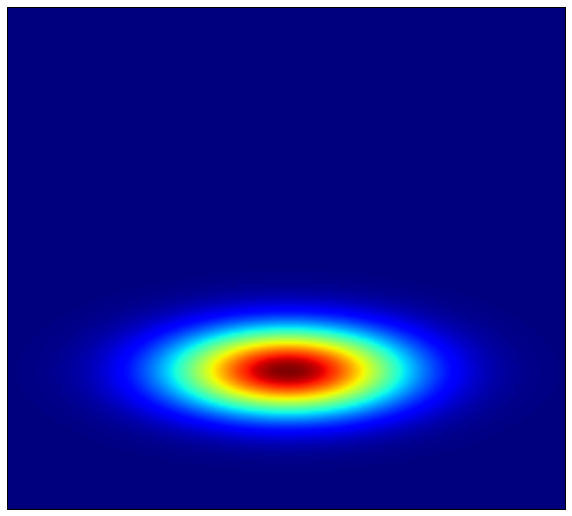
\includegraphics[width=10cm]{2c1.png}
\subsubsection{}
\eqar{
  \angl{N'}=&\angl{\paren{ta^\dagger+rb^\dagger}\paren{ta+rb}}\\
  =&\angl{t^2n_a+r^2n_b}\\
  =&TN_a+\paren{1-T}N_b
}
\subsubsection{}
\eqar{
  \Delta n'^2=&\angl{n'^2}-\angl{n'}^2\\
  =&\angl{\paren{\paren{ta^\dagger+rb^\dagger}\paren{ta+rb}}^2}-\angl{\paren{ta^\dagger+rb^\dagger}\paren{ta+rb}}^2\\
  =&\angl{\paren{t^2n_a+r^2n_b+tr\paren{a^\dagger b+b^\dagger a}}^2}-\paren{TN_a+RN_b}^2\\
  =&T^2\Delta N_a^2+R^2\Delta N_b^2+TR\angl{\paren{a^\dagger\beta+\beta^*a}^2}
  \intertext{For large $N_a$ and if the displacement is along the lower variant direction}
  \Delta n'^2\approx&T^2\Delta N_a^2+R^2\Delta N_b^2
}
\subsubsection{}
\eqar{
  \Delta n'^2\approx&2T^2N_a^2+R^2 N_b
  \intertext{In order to be smaller than $\angl{N'}$}
  N_b>&\frac{\paren{2TN_a-1}N_a}{R}
  \intertext{And the squeezing should be strong enough that $2TN_a>1$}
}

\section{}
\subsection{}
\eqar{
  a_{out}=&\frac{a_2-b_2}{\sqrt{2}}\\
  =&\frac{a_1\ue^{\ui\varphi}-b_1}{\sqrt{2}}\\
  =&\frac{1}{2}\paren{\paren{a-b}\ue^{\ui\varphi}-a-b}\\
  =&\ue^{\ui\varphi/2}\paren{\ui a\sin\frac{\varphi}{2}-b\cos\frac{\varphi}{2}}\\
  a_{out}^\dagger=&\ue^{-\ui\varphi/2}\paren{-\ui a^\dagger\sin\frac{\varphi}{2}-b^\dagger\cos\frac{\varphi}{2}}
  \intertext{}
  b_{out}=&\frac{a_2+b_2}{\sqrt{2}}\\
  =&\frac{a_1\ue^{\ui\varphi}+b_1}{\sqrt{2}}\\
  =&\frac{1}{2}\paren{\paren{a-b}\ue^{\ui\varphi}+a+b}\\
  =&\ue^{\ui\varphi/2}\paren{a\cos\frac{\varphi}{2}-\ui b\sin\frac{\varphi}{2}}\\
  b_{out}^\dagger=&\ue^{-\ui\varphi/2}\paren{a^\dagger\cos\frac{\varphi}{2}+\ui b^\dagger\sin\frac{\varphi}{2}}
  \intertext{}
  n_{out_a}=&\paren{-\ui a^\dagger\sin\frac{\varphi}{2}-b^\dagger\cos\frac{\varphi}{2}}\paren{\ui a\sin\frac{\varphi}{2}-b\cos\frac{\varphi}{2}}\\
  =&n_a\sin^2\frac{\varphi}{2}+n_b\cos^2\frac{\varphi}{2}+\ui\sin\frac{\varphi}{2}\cos\frac{\varphi}{2}\paren{a^\dagger b-ab^\dagger}
  \intertext{}
  n_{out_b}=&\paren{a^\dagger\cos\frac{\varphi}{2}+\ui b^\dagger\sin\frac{\varphi}{2}}\paren{a\cos\frac{\varphi}{2}-\ui b\sin\frac{\varphi}{2}}\\
  =&n_a\cos^2\frac{\varphi}{2}+n_b\sin^2\frac{\varphi}{2}+\ui\sin\frac{\varphi}{2}\cos\frac{\varphi}{2}\paren{ab^\dagger-a^\dagger b}
  \intertext{}
  &b_{out}^\dagger b_{out}-a_{out}^\dagger a_{out}\\
  =&n_a\cos\varphi-n_b\cos\varphi+\ui\sin\varphi\paren{ab^\dagger-a^\dagger b}\\
  \intertext{Average}
  &\angl{b_{out}^\dagger b_{out}-a_{out}^\dagger a_{out}}\\
  =&\angl{n_a\cos\varphi}\\
  =&\abs{\alpha}^2\cos\varphi
  \intertext{Square}
  &\angl{\paren{b_{out}^\dagger b_{out}-a_{out}^\dagger a_{out}}^2}\\
  =&\angl{\paren{n_a\cos\varphi-n_b\cos\varphi+\ui\sin\varphi\paren{ab^\dagger-a^\dagger b}}\paren{n_a\cos\varphi-n_b\cos\varphi+\ui\sin\varphi\paren{ab^\dagger-a^\dagger b}}}\\
  =&\angl{\paren{n_a\cos\varphi-\ui\sin\varphi\alpha^*b}\paren{n_a\cos\varphi+\ui\sin\varphi\alpha b^\dagger}}\\
  =&\cos^2\varphi\angl{n_a}^2+\abs{\alpha}^2\sin^2\varphi\\
  \intertext{Fluctuation}
  &\Delta\paren{b_{out}^\dagger b_{out}-a_{out}^\dagger a_{out}}^2\\
  =&\cos^2\varphi\Delta n_a^2+\abs{\alpha}^2\sin^2\varphi\\
  =&\abs{\alpha}^2\\
  SNR=&\frac{\abs{\alpha}^2\cos\varphi}{\abs{\alpha}}\\
  =&\abs{\alpha}\cos\varphi
}
\subsection{}
$\varphi'=\dfrac\pi2-\varphi$
\eqar{
  SNR\approx&\abs{\alpha}\varphi'\\
  \varphi'_{min}=&\frac{1}{\abs{\alpha}}
}
\subsection{}
Average
\eqar{
  &b_{out}^\dagger b_{out}-a_{out}^\dagger a_{out}\\
  =&n_a\cos\varphi-\paren{t^\dagger\cosh\varepsilon-t\sinh\varepsilon}\paren{t\cosh\varepsilon-t^\dagger\sinh\varepsilon}\cos\varphi\\
  &+\ui\sin\varphi\paren{a\paren{t^\dagger\cosh\varepsilon-t\sinh\varepsilon}-a^\dagger\paren{t\cosh\varepsilon-t^\dagger\sinh\varepsilon}}\\
  =&n_a\cos\varphi-\cos\varphi\paren{
    \cosh2\varepsilon n_t+\sinh^2\varepsilon
    -\sinh\varepsilon\cosh\varepsilon\paren{{t^\dagger}^2+t^2}}\\
  &+\ui\sin\varphi\paren{a\paren{t^\dagger\cosh\varepsilon-t\sinh\varepsilon}-a^\dagger\paren{t\cosh\varepsilon-t^\dagger\sinh\varepsilon}}\\
  &\angl{b_{out}^\dagger b_{out}-a_{out}^\dagger a_{out}}\\
  =&\langle
  n_a\cos\varphi-\cos\varphi\paren{
    \cosh2\varepsilon n_t+\sinh^2\varepsilon
    -\sinh\varepsilon\cosh\varepsilon\paren{{t^\dagger}^2+t^2}}\\
  &+\ui\sin\varphi\paren{a\paren{t^\dagger\cosh\varepsilon-t\sinh\varepsilon}-a^\dagger\paren{t\cosh\varepsilon-t^\dagger\sinh\varepsilon}}
  \rangle\\
  =&\abs{\alpha}^2\cos\varphi-\cos\varphi\sinh^2\varepsilon
  \intertext{Square}
  &\angl{\paren{b_{out}^\dagger b_{out}-a_{out}^\dagger a_{out}}^2}\\
  =&\langle
  \left(n_a\cos\varphi-\cos\varphi\paren{
      \cosh2\varepsilon n_t+\sinh^2\varepsilon
      -\sinh\varepsilon\cosh\varepsilon\paren{{t^\dagger}^2+t^2}}\right.\\
  &\left.+\ui\sin\varphi\paren{a\paren{t^\dagger\cosh\varepsilon-t\sinh\varepsilon}-a^\dagger\paren{t\cosh\varepsilon-t^\dagger\sinh\varepsilon}}\right)\\
  &\left(n_a\cos\varphi-\cos\varphi\paren{
      \cosh2\varepsilon n_t+\sinh^2\varepsilon
      -\sinh\varepsilon\cosh\varepsilon\paren{{t^\dagger}^2+t^2}}\right.\\
  &\left.+\ui\sin\varphi\paren{a\paren{t^\dagger\cosh\varepsilon-t\sinh\varepsilon}-a^\dagger\paren{t\cosh\varepsilon-t^\dagger\sinh\varepsilon}}\right)
  \rangle\\
  =&\langle
  \paren{n_a\cos\varphi-\cos\varphi\paren{
      \sinh^2\varepsilon-\sinh\varepsilon\cosh\varepsilon t^2}-\ui t\sin\varphi\paren{a\sinh\varepsilon+a^\dagger\cosh\varepsilon}}\\
  &\paren{n_a\cos\varphi-\cos\varphi\paren{
      \sinh^2\varepsilon-\sinh\varepsilon\cosh\varepsilon{t^\dagger}^2}
    +\ui\sin\varphi t^\dagger\paren{a\cosh\varepsilon+a^\dagger\sinh\varepsilon}}
  \rangle\\
  =&\langle
  \paren{n_a\cos\varphi-\cos\varphi\sinh^2\varepsilon
    +\cos\varphi\sinh\varepsilon\cosh\varepsilon t^2-\ui t\sin\varphi\paren{a\sinh\varepsilon+\alpha^*\cosh\varepsilon}}\\
  &\paren{n_a\cos\varphi-\cos\varphi\sinh^2\varepsilon
    +\cos\varphi\sinh\varepsilon\cosh\varepsilon{t^\dagger}^2
    +\ui t^\dagger\sin\varphi\paren{\alpha\cosh\varepsilon+a^\dagger\sinh\varepsilon}}
  \rangle\\
  =&\angl{\paren{n_a\cos\varphi-\cos\varphi\sinh^2\varepsilon}^2}+\langle
  \cos^2\varphi\sinh^2\varepsilon\cosh^2\varepsilon tt^\dagger tt^\dagger
  \rangle\\
  &+\langle
  \paren{\cos\varphi\sinh\varepsilon\cosh\varepsilon t-\ui\sin\varphi\paren{a\sinh\varepsilon+\alpha^*\cosh\varepsilon}}\\
  &\paren{\cos\varphi\sinh\varepsilon\cosh\varepsilon{t^\dagger}
    +\ui\sin\varphi\paren{\alpha\cosh\varepsilon+a^\dagger\sinh\varepsilon}}
  \rangle\\
  =&\angl{\paren{n_a\cos\varphi-\cos\varphi\sinh^2\varepsilon}^2}
  +2\cos^2\varphi\sinh^2\varepsilon\cosh^2\varepsilon\\
  &+\sin^2\varphi\abs{\alpha\sinh\varepsilon+\alpha^*\cosh\varepsilon}^2
  +\sin^2\varphi\sinh^2\varepsilon
  \intertext{Fluctuation}
  &\Delta\paren{b_{out}^\dagger b_{out}-a_{out}^\dagger a_{out}}^2\\
  =&\abs{\alpha}^2\cos^2\varphi
  +2\cos^2\varphi\sinh^2\varepsilon\cosh^2\varepsilon
  +\sin^2\varphi\abs{\alpha\sinh\varepsilon+\alpha^*\cosh\varepsilon}^2
  +\sin^2\varphi\sinh^2\varepsilon\\
  \approx&\abs{\alpha}^2\varphi'^2
  +2\varphi^2\sinh^2\varepsilon\cosh^2\varepsilon
  +\paren{1-\varphi^2}\abs{\alpha\sinh\varepsilon+\alpha^*\cosh\varepsilon}^2
  +\paren{1-\varphi^2}\sinh^2\varepsilon
}
Minimum angle
\eqar{
  \varphi'^2\paren{\abs{\alpha}^2-\sinh^2\varepsilon}^2=&\abs{\alpha}^2\varphi'^2
  +2\varphi'^2\sinh^2\varepsilon\cosh^2\varepsilon
  +\paren{1-\varphi'^2}\abs{\alpha\sinh\varepsilon+\alpha^*\cosh\varepsilon}^2
  +\paren{1-\varphi'^2}\sinh^2\varepsilon
  \intertext{In high power limit}
  \varphi'^2\abs{\alpha}^4=&\abs{\alpha\sinh\varepsilon+\alpha^*\cosh\varepsilon}^2
  \intertext{To get a factor of $\beta$ in phase resolution}
  \frac{\alpha^2}{\beta^2}=&\abs{\alpha\sinh\varepsilon+\alpha^*\cosh\varepsilon}^2
  \intertext{With correct phase of $\alpha$}
  \beta=&\ue^{\varepsilon}\\
  \varepsilon=&\ln\beta
}
Squeezing changes the photon number because squeezed vacuum has non-zero photon number.

\subsection{}
For coherent state
\eqar{
  \alpha=&\sqrt{\frac{PL\lambda}{\pi\hbar c^2}}\\
  =&2.7\cdot10^7\\
  \varphi_{min}=&3.7\cdot10^{-8}\\
  l_{min}=&6.3\cdot10^{-15}m\\
  \varepsilon_{min}=&1.6\cdot10^{-18}
  \intertext{With a $6$dB squeezed vaccum, the sensitivity can go up by a factor of $4$}
}

\end{document}
